% I seguenti commenti speciali impostano:
% 1. 
% 2. PDFLaTeX come motore di composizione;
% 3. tesi.tex come documento principale;
% 4. il controllo ortografico italiano per l'editor.

% !TEX encoding = UTF-8
% !TEX TS-program = pdflatex
% !TEX root = tesi.tex
% !TEX spellcheck = it-IT

\documentclass[10pt,                    % corpo del font principale
               a4paper,                 % carta A4
               twoside,                 % impagina per fronte-retro
               openright,               % inizio capitoli a destra
               english,                 
               italian,                 
               ]{book}    

\usepackage[utf8]{inputenc}             % codifica di input; anche [latin1] va bene
                                        % NOTA BENE! va accordata con le preferenze dell'editor

%**************************************************************
% Importazione package
%************************************************************** 

%\usepackage{amsmath,amssymb,amsthm}    % matematica

\usepackage[english, italian]{babel}    % per scrivere in italiano e in inglese;
                                        % l'ultima lingua (l'italiano) risulta predefinita

\usepackage{bookmark}                   % segnalibri

\usepackage{caption}                    % didascalie

\usepackage{chngpage,calc}              % centra il frontespizio

\usepackage{csquotes}                   % gestisce automaticamente i caratteri (")

\usepackage{emptypage}                  % pagine vuote senza testatina e piede di pagina

\usepackage{epigraph}					% per epigrafi

\usepackage{eurosym}                    % simbolo dell'euro

\usepackage[T1]{fontenc}                % codifica dei font:
                                        % NOTA BENE! richiede una distribuzione *completa* di LaTeX

%\usepackage{indentfirst}               % rientra il primo paragrafo di ogni sezione

\usepackage{graphicx}                   % immagini

\usepackage{hyperref}                   % collegamenti ipertestuali



\usepackage[binding=5mm]{layaureo}      % margini ottimizzati per l'A4; rilegatura di 5 mm

\usepackage{listings}                   % codici

\usepackage{microtype}                  % microtipografia

\usepackage{mparhack,fixltx2e,relsize}  % finezze tipografiche

\usepackage{nameref}                    % visualizza nome dei riferimenti                                      

\usepackage[font=small]{quoting}        % citazioni

\usepackage{subfig}                     % sottofigure, sottotabelle

\usepackage[italian]{varioref}          % riferimenti completi della pagina

\usepackage[dvipsnames]{xcolor}         % colori

\usepackage{booktabs}                   % tabelle                                       
\usepackage{tabularx}                   % tabelle di larghezza prefissata                                    
\usepackage{longtable}                  % tabelle su più pagine                                        
\usepackage{ltxtable}                   % tabelle su più pagine e adattabili in larghezza

\usepackage[toc, acronym]{glossaries}   % glossario
                                        % per includerlo nel documento bisogna:
                                        % 1. compilare una prima volta tesi.tex;
                                        % 2. eseguire: makeindex -s tesi.ist -t tesi.glg -o tesi.gls tesi.glo
                                        % 3. eseguire: makeindex -s tesi.ist -t tesi.alg -o tesi.acr tesi.acn
                                        % 4. compilare due volte tesi.tex.

\usepackage[backend=biber,style=verbose-ibid,hyperref,backref]{biblatex}
                                        % eccellente pacchetto per la bibliografia; 
                                        % produce uno stile di citazione autore-anno; 
                                        % lo stile "numeric-comp" produce riferimenti numerici
                                        % per includerlo nel documento bisogna:
                                        % 1. compilare una prima volta tesi.tex;
                                        % 2. eseguire: biber tesi
                                        % 3. compilare ancora tesi.tex.

%**************************************************************
% file contenente le impostazioni della tesi
%**************************************************************

%**************************************************************
% Frontespizio
%**************************************************************
\newcommand{\myName}{Stefano Campese}                                    % autore
\newcommand{\myTitle}{Lactobacillus Casei resequencing}                    
\newcommand{\myDegree}{Bioinformatics project}                % tipo di tesi
\newcommand{\myUni}{University of Padova}           % università
\newcommand{\myFaculty}{Master degree in Computer Science}         % facoltà
\newcommand{\myDepartment}{Math departement}          % dipartimento
\newcommand{\myProf}{Giorgio Valle}                                % relatore
\newcommand{\myLocation}{Padova}                                % dove
\newcommand{\myAA}{2015-2016}                                   % anno accademico
\newcommand{\myTime}{Feb 2016}                                  % quando


%**************************************************************
% Impostazioni di impaginazione
% see: http://wwwcdf.pd.infn.it/AppuntiLinux/a2547.htm
%**************************************************************

\setlength{\parindent}{14pt}   % larghezza rientro della prima riga
\setlength{\parskip}{0pt}   % distanza tra i paragrafi


%**************************************************************
% Impostazioni di biblatex
%**************************************************************
\bibliography{bibliografia} % database di biblatex 

\defbibheading{bibliography}
{
    \cleardoublepage
    \phantomsection 
    \addcontentsline{toc}{chapter}{\bibname}
    \chapter*{\bibname\markboth{\bibname}{\bibname}}
}

\setlength\bibitemsep{1.5\itemsep} % spazio tra entry

\DeclareBibliographyCategory{opere}
\DeclareBibliographyCategory{web}

\addtocategory{opere}{womak:lean-thinking}
\addtocategory{web}{site:agile-manifesto}

\defbibheading{opere}{\section*{Riferimenti bibliografici}}
\defbibheading{web}{\section*{Siti Web consultati}}


%**************************************************************
% Impostazioni di caption
%**************************************************************
\captionsetup{
    tableposition=top,
    figureposition=bottom,
    font=small,
    format=hang,
    labelfont=bf
}

%**************************************************************
% Impostazioni di glossaries
%**************************************************************

%**************************************************************
% Acronimi
%**************************************************************
\renewcommand{\acronymname}{Acronimi e abbreviazioni}

\newacronym[description={\glslink{apig}{Application Program Interface}}]
    {api}{API}{Application Program Interface}

\newacronym[description={\glslink{umlg}{Unified Modeling Language}}]
    {uml}{UML}{Unified Modeling Language}

%**************************************************************
% Glossario
%**************************************************************
%\renewcommand{\glossaryname}{Glossario}

\newglossaryentry{apig}
{
    name=\glslink{api}{API},
    text=Application Program Interface,
    sort=api,
    description={in informatica con il termine \emph{Application Programming Interface API} (ing. interfaccia di programmazione di un'applicazione) si indica ogni insieme di procedure disponibili al programmatore, di solito raggruppate a formare un set di strumenti specifici per l'espletamento di un determinato compito all'interno di un certo programma. La finalità è ottenere un'astrazione, di solito tra l'hardware e il programmatore o tra software a basso e quello ad alto livello semplificando così il lavoro di programmazione}
}

\newglossaryentry{umlg}
{
    name=\glslink{uml}{UML},
    text=UML,
    sort=uml,
    description={in ingegneria del software \emph{UML, Unified Modeling Language} (ing. linguaggio di modellazione unificato) è un linguaggio di modellazione e specifica basato sul paradigma object-oriented. L'\emph{UML} svolge un'importantissima funzione di ``lingua franca'' nella comunità della progettazione e programmazione a oggetti. Gran parte della letteratura di settore usa tale linguaggio per descrivere soluzioni analitiche e progettuali in modo sintetico e comprensibile a un vasto pubblico}
}
 % database di termini
\makeglossaries


%**************************************************************
% Impostazioni di graphicx
%**************************************************************
\graphicspath{{immagini/}} % cartella dove sono riposte le immagini


%**************************************************************
% Impostazioni di hyperref
%**************************************************************
\hypersetup{
    %hyperfootnotes=false,
    %pdfpagelabels,
    %draft,	% = elimina tutti i link (utile per stampe in bianco e nero)
    colorlinks=true,
    linktocpage=true,
    pdfstartpage=1,
    pdfstartview=FitV,
    % decommenta la riga seguente per avere link in nero (per esempio per la stampa in bianco e nero)
    %colorlinks=false, linktocpage=false, pdfborder={0 0 0}, pdfstartpage=1, pdfstartview=FitV,
    breaklinks=true,
    pdfpagemode=UseNone,
    pageanchor=true,
    pdfpagemode=UseOutlines,
    plainpages=false,
    bookmarksnumbered,
    bookmarksopen=true,
    bookmarksopenlevel=1,
    hypertexnames=true,
    pdfhighlight=/O,
    %nesting=true,
    %frenchlinks,
    urlcolor=webbrown,
    linkcolor=RoyalBlue,
    citecolor=webgreen,
    %pagecolor=RoyalBlue,
    %urlcolor=Black, linkcolor=Black, citecolor=Black, %pagecolor=Black,
    pdftitle={\myTitle},
    pdfauthor={\textcopyright\ \myName, \myUni, \myFaculty},
    pdfsubject={},
    pdfkeywords={},
    pdfcreator={pdfLaTeX},
    pdfproducer={LaTeX}
}

%**************************************************************
% Impostazioni di itemize
%**************************************************************
\renewcommand{\labelitemi}{$\ast$}

%\renewcommand{\labelitemi}{$\bullet$}
%\renewcommand{\labelitemii}{$\cdot$}
%\renewcommand{\labelitemiii}{$\diamond$}
%\renewcommand{\labelitemiv}{$\ast$}


%**************************************************************
% Impostazioni di listings
%**************************************************************
\lstset{
    language=[LaTeX]Tex,%C++,
    keywordstyle=\color{RoyalBlue}, %\bfseries,
    basicstyle=\small\ttfamily,
    %identifierstyle=\color{NavyBlue},
    commentstyle=\color{Green}\ttfamily,
    stringstyle=\rmfamily,
    numbers=none, %left,%
    numberstyle=\scriptsize, %\tiny
    stepnumber=5,
    numbersep=8pt,
    showstringspaces=false,
    breaklines=true,
    frameround=ftff,
    frame=single
} 


%**************************************************************
% Impostazioni di xcolor
%**************************************************************
\definecolor{webgreen}{rgb}{0,.5,0}
\definecolor{webbrown}{rgb}{.6,0,0}


%**************************************************************
% Altro
%**************************************************************

\newcommand{\omissis}{[\dots\negthinspace]} % produce [...]

% eccezioni all'algoritmo di sillabazione
\hyphenation
{
    ma-cro-istru-zio-ne
    gi-ral-din
}

\newcommand{\sectionname}{sezione}
\addto\captionsitalian{\renewcommand{\figurename}{figura}
                       \renewcommand{\tablename}{tabella}}

\newcommand{\glsfirstoccur}{\ap{{[g]}}}

\newcommand{\intro}[1]{\emph{\textsf{#1}}}

%**************************************************************
% Environment per ``rischi''
%**************************************************************
\newcounter{riskcounter}                % define a counter
\setcounter{riskcounter}{0}             % set the counter to some initial value

%%%% Parameters
% #1: Title
\newenvironment{risk}[1]{
    \refstepcounter{riskcounter}        % increment counter
    \par \noindent                      % start new paragraph
    \textbf{\arabic{riskcounter}. #1}   % display the title before the 
                                        % content of the environment is displayed 
}{
    \par\medskip
}

\newcommand{\riskname}{Rischio}

\newcommand{\riskdescription}[1]{\textbf{\\Descrizione:} #1.}

\newcommand{\risksolution}[1]{\textbf{\\Soluzione:} #1.}

%**************************************************************
% Environment per ``use case''
%**************************************************************
\newcounter{usecasecounter}             % define a counter
\setcounter{usecasecounter}{0}          % set the counter to some initial value

%%%% Parameters
% #1: ID
% #2: Nome
\newenvironment{usecase}[2]{
    \renewcommand{\theusecasecounter}{\usecasename #1}  % this is where the display of 
                                                        % the counter is overwritten/modified
    \refstepcounter{usecasecounter}             % increment counter
    \vspace{10pt}
    \par \noindent                              % start new paragraph
    {\large \textbf{\usecasename #1: #2}}       % display the title before the 
                                                % content of the environment is displayed 
    \medskip
}{
    \medskip
}

\newcommand{\usecasename}{UC}

\newcommand{\usecaseactors}[1]{\textbf{\\Attori Principali:} #1. \vspace{4pt}}
\newcommand{\usecasepre}[1]{\textbf{\\Precondizioni:} #1. \vspace{4pt}}
\newcommand{\usecasedesc}[1]{\textbf{\\Descrizione:} #1. \vspace{4pt}}
\newcommand{\usecasepost}[1]{\textbf{\\Postcondizioni:} #1. \vspace{4pt}}
\newcommand{\usecasealt}[1]{\textbf{\\Scenario Alternativo:} #1. \vspace{4pt}}

%**************************************************************
% Environment per ``namespace description''
%**************************************************************

\newenvironment{namespacedesc}{
    \vspace{10pt}
    \par \noindent                              % start new paragraph
    \begin{description} 
}{
    \end{description}
    \medskip
}

\newcommand{\classdesc}[2]{\item[\textbf{#1:}] #2}
                     % file con le impostazioni personali

\begin{document}
%**************************************************************
% Materiale iniziale
%**************************************************************
\frontmatter
% !TEX encoding = UTF-8
% !TEX TS-program = pdflatex
% !TEX root = ../tesi.tex
% !TEX spellcheck = it-IT

%**************************************************************
% Frontespizio 
%**************************************************************
\begin{titlepage}

\begin{center}

\begin{LARGE}
\textbf{\myUni}\\
\end{LARGE}

\vspace{10pt}

\begin{Large}
\textsc{\myDepartment}\\
\end{Large}

\vspace{10pt}

\begin{large}
\textsc{\myFaculty}\\
\end{large}

\vspace{30pt}
\begin{figure}[htbp]
\begin{center}

\includegraphics[height=6cm]{logo-unipd}
\end{center}
\end{figure}
\vspace{30pt} 

\begin{LARGE}
\begin{center}
\textbf{\myTitle}\\
\end{center}
\end{LARGE}

\vspace{10pt} 

\begin{large}
\textsl{\myDegree}\\
\end{large}

\vspace{40pt} 

\begin{large}
\begin{flushleft}
%\textit{Relatore}\\ 
\vspace{5pt} 
Prof. \myProf
\end{flushleft}

\vspace{0pt} 

\begin{flushright}
%\textit{Laureando}\\ 
\vspace{5pt} 
\myName
\end{flushright}
\end{large}

\vspace{40pt}

\line(1, 0){338} \\
\begin{normalsize}
\textsc{Anno Accademico \myAA}
\end{normalsize}

\end{center}
\end{titlepage} 
%% !TEX encoding = UTF-8
% !TEX TS-program = pdflatex
% !TEX root = ../tesi.tex
% !TEX spellcheck = it-IT

%**************************************************************
% Colophon
%**************************************************************
\clearpage
\phantomsection
\thispagestyle{empty}

\hfill

\vfill

\noindent\myName: \textit{\myTitle,}
\myDegree,
\textcopyright\ \myTime.
%% !TEX encoding = UTF-8
% !TEX TS-program = pdflatex
% !TEX root = ../tesi.tex
% !TEX spellcheck = it-IT

%**************************************************************
% Dedica
%**************************************************************
\cleardoublepage
\phantomsection
\thispagestyle{empty}
\pdfbookmark{Dedica}{Dedica}

\vspace*{3cm}

\begin{center}
Lorem ipsum dolor sit amet, consectetuer adipiscing elit. \\ \medskip
--- Oscar Wilde    
\end{center}

\medskip

\begin{center}
Dedicato a ...
\end{center}

%% !TEX encoding = UTF-8
% !TEX TS-program = pdflatex
% !TEX root = ../tesi.tex
% !TEX spellcheck = it-IT

%**************************************************************
% Sommario
%**************************************************************
\cleardoublepage
\phantomsection
\pdfbookmark{Sommario}{Sommario}
\begingroup
\let\clearpage\relax
\let\cleardoublepage\relax
\let\cleardoublepage\relax

\chapter*{Sommario}

Il presente documento descrive il lavoro svolto durante il periodo di stage, della durata di circa trecento ore, dal laureando Pinco Pallino presso l'azienda Azienda S.p.A.
Gli obbiettivi da raggiungere erano molteplici.\\
In primo luogo era richiesto lo sviluppo di ...
In secondo luogo era richiesta l'implementazione di un ... 
Tale framework permette di registrare gli eventi di un controllore programmabile, quali segnali applicati 
Terzo ed ultimo obbiettivo era l'integrazione ...

%\vfill
%
%\selectlanguage{english}
%\pdfbookmark{Abstract}{Abstract}
%\chapter*{Abstract}
%
%\selectlanguage{italian}

\endgroup			

\vfill


%% !TEX encoding = UTF-8
% !TEX TS-program = pdflatex
% !TEX root = ../tesi.tex
% !TEX spellcheck = it-IT

%**************************************************************
% Ringraziamenti
%**************************************************************
\cleardoublepage
\phantomsection
\pdfbookmark{Ringraziamenti}{ringraziamenti}

\begin{flushright}{
	\slshape    
	``Life is really simple, but we insist on making it complicated''} \\ 
	\medskip
    --- Confucius
\end{flushright}


\bigskip

\begingroup
\let\clearpage\relax
\let\cleardoublepage\relax
\let\cleardoublepage\relax

\chapter*{Ringraziamenti}

\noindent \textit{Innanzitutto, vorrei esprimere la mia gratitudine al Prof. NomeDelProfessore, relatore della mia tesi, per l'aiuto e il sostegno fornitomi durante la stesura del lavoro.}\\

\noindent \textit{Desidero ringraziare con affetto i miei genitori per il sostegno, il grande aiuto e per essermi stati vicini in ogni momento durante gli anni di studio.}\\

\noindent \textit{Ho desiderio di ringraziare poi i miei amici per tutti i bellissimi anni passati insieme e le mille avventure vissute.}\\
\bigskip

\noindent\textit{\myLocation, \myTime}
\hfill \myName

\endgroup


% !TEX encoding = UTF-8
% !TEX TS-program = pdflatex
% !TEX root = ../tesi.tex
% !TEX spellcheck = it-IT

%**************************************************************
% Indici
%**************************************************************
\cleardoublepage
\pdfbookmark{\contentsname}{tableofcontents}
\setcounter{tocdepth}{2}
\tableofcontents
%\markboth{\contentsname}{\contentsname} 
\clearpage

\begingroup 
    \let\clearpage\relax
    \let\cleardoublepage\relax
    \let\cleardoublepage\relax
    %*******************************************************
    % Elenco delle figure
    %*******************************************************    
    \phantomsection
    \pdfbookmark{\listfigurename}{lof}
    \listoffigures

       
    \vspace*{8ex}
\endgroup

\cleardoublepage

\cleardoublepage

%**************************************************************
% Materiale principale
%**************************************************************
\mainmatter
% !TEX encoding = UTF-8
% !TEX TS-program = pdflatex
% !TEX root = ../tesi.tex
% !TEX spellcheck = it-IT

%**************************************************************
\chapter{Resequencing}
\label{cap:resequencing}
%**************************************************************

For the project development a bacterial genome was provided\\

This genome belongs to \emph{Lactobacillus casei} and it is quite long genome, 3.079.196 long bases.

The goal of the project is sequence a similar bacterium, defined as sample (or test), using the mate pairs that derived from it, to find and highlight any structural variation as inversions, deletions or insertions.\\
In particular, the tracks are to be produced displayable on Integrative Genome Browser (IGV).
The project includes a part of data analysis to understand the nature and a programming part for the production of results.

%**************************************************************
\section{Instruments}

I used these instruments:
\begin{itemize}
\item IGV that allows the displayment of traks on reference genome.
\item BWA for the alignment of the mate pairs on reference genome.
\item R for the traks plotting
\end{itemize}

For the algorithms development, Python 3 was used.

%**************************************************************
\section{Datas}

For development of the project, the given datas are:\\
    

\begin{itemize}
\item \begin{description}
		\item[Lactobacillus\_caei\_genome.fasta:] the genome of the bacterium
	  \end{description}
\end{itemize}

\begin{itemize}
\item \begin{description}
		\item[lact\_sp\_read1.fastaq:] the first reads of resequencing
	  \end{description}
\end{itemize}

\begin{itemize}
\item \begin{description}
		\item[lact\_sp\_read12.fastaq:] the second reads of resequencing
	  \end{description}
\end{itemize}
  
These last two files contains the reads, the quality of each base of the reads and others useful information that allows the SAM file creation.

From the SAM file I extracted and used some different datas as:

\begin{itemize}
\item \begin{description}
		\item[FLAG:] It provides information related to matching the rid or mate pair. In case of simple alignment without pairing, this value is useful to see if the read is aligned on the positive or negative strand.
	  \end{description}
\end{itemize}


\begin{itemize}
\item \begin{description}
		\item[POS:] position where is aligned the read or mate
		  \end{description}
\end{itemize}

\begin{itemize}
\item \begin{description}
		\item[CIGAR:] how and the kind of the alignement. This field also tell how each base is algined/deleted/inserted or others
  \end{description}
\end{itemize}
\begin{itemize}
\item \begin{description}
		\item[TLEN:] length of mate-pair
		  \end{description}
\end{itemize}
\begin{itemize}
\item \begin{description}
		\item[SEQ:] sequence of bases that make up the read
  \end{description}
\end{itemize}


%**************************************************************
\section{Results}

The results of the project, are composed by wig files ( plain text ), tdf files ( pre digested binary file for IGV, that come from wig files ), csv files ( for statistical manipulation ) and also png file for the data's traks.\\\\

The algorithms, as output, generate the wig files that are converted to tdf files by IGV tools.\\\\

Some results, as the \emph{barchart trak} of the genome insertion lenght, are obtained by passing a csv file, that is generated by algorithm, to a R script that plot and create images.             % Introduzione
% !TEX encoding = UTF-8
% !TEX TS-program = pdflatex
% !TEX root = ../tesi.tex
% !TEX spellcheck = it-IT

%**************************************************************
\chapter{Project Development}
\label{cap:project-development}
%**************************************************************

\intro{Brevissima introduzione al capitolo}\\

%**************************************************************
\section{SAM file creation}
At first time, to procede with the project, I've created the SAM file by using the \emph{Burrows-Wheeler Aligner} supplied by BWA.
The software could be found here: \href{http://bio-bwa.sourceforge.net}[http://bio-bwa.sourceforge.net]

The first command necessary for the file creation is:
\\
\\
\verb|bwa index Lactobacillus_casei_genome.fasta|
\\
\\
This command serves to index the fasta genome file. The indexing of the genome's file allows the increasing of the performance during the genome alignment phase.\\

The second typed command is:
\\
\\
\verb|bwa mem Lactobacillus_casei_genome.fasta lact_sp.read1.fastq lact_sp.read2.fastq > Lactobacillus_casei_genome.sam|
\\
\\
This command allows the alignment of the two reads files on the reference genome file into a SAM file that servers for the project.\\

There are others different instruments that made this, but BWA should be the best tools specially for the performance.\\

The goal file contains all the informations about the resequenced genome in according with the SAM specifications.
It weight of the file is more or less 890MB.


\section{Insertion length}
For this point I wrote an algorithm, that for each row of the SAM file, which contains information about the resequencing, extract the value obtained from :
\\
\\
\verb|abs(POS -PNEXT)|
\\
\\
Where \emph{POS} is the start of the read and \emph{PNEXT} is the start position of the next read.\\
For research fo the insert size length, there are some different opinion that comes from different sources, some of these suggests to use only the \emph{TLEN} field of the SAM file to calculate the insert size length.
\\\\
Once time that I extracted all the insertion length, I plotted all the data in a BatChart trak, as yuo could see here \ref{fig:1}.\\
This trak allows to identify the wrong lectures and the wrong reads.
\\\\
For this trak, a R script was made; from this chart, as I already wrote, is possible to analize the reads that has wrong insert values, which in some cases, is over 2 milion bases long.\\

This error could be partially explained by the multiple alignment of the reads on reference genome.

 \begin{figure}[H]
				\centering
				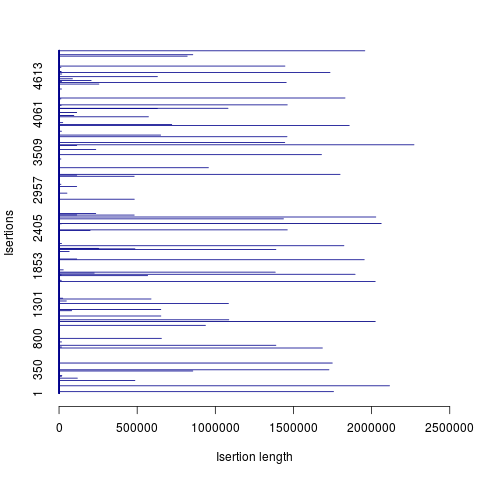
\includegraphics[scale=0.8]{immagini/r.png}
				\caption{Barchart for the isize without exluding errors, the chart include only the first 10.000 reads}\label{fig:1}
				\end{figure}

From this trak, is possibile to see how some read that has the insert lenght longer then 10.000 bases has an error, so for the mean and the standard deviation, this read was be exluded.
Here \ref{fig:2} you could see the trak that exlude the reads with insert equal to or greather then 10.000 bases long. The obtained chart is more right then first chart.
 \begin{figure}[H]
				\centering
				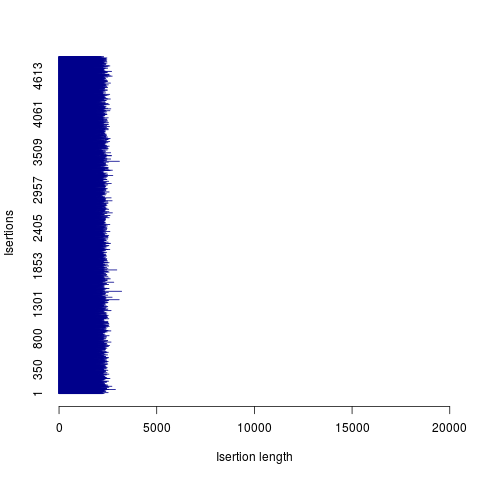
\includegraphics[scale=0.8]{immagini/r1.png}
				\caption{Barchart for the isize without errors}\label{fig:2}
				\end{figure}

The result of mean and standard deviation are:
\begin{itemize}
\item \begin{description}
		\item[MEAN:] 2102
  \end{description}
\end{itemize}

\begin{itemize}
\item \begin{description}
		\item[STD:] 236.84
  \end{description}
\end{itemize}


The result of this point, also, is a csv file that allows to create a barchart with the insertions size with the R script.

\section{Physical Coverage}

The Physical Coverage is calulated by an algorithm really similar to the given Perl script.\\

The mainly reason is the optimization of the algorithm.\\\\

The algorithm, infact, loops on half of reads by checking if the \emph{TLEN} is greather then 0.\\
At first time, I had created an array where each cell was be intialized to 0. 
In each one of these cells, I putted +1 when the index is equal to the read start position, and I putted -1 when the index is equal to the next read start position.\\

Is necessary mentioning which the used reads, are only the right aligned reads, and the filtering of the right-wrong reads is made by checking the \emph{FLAG} field of the SAM file.
\\
The resultant values are putted inside a wig file, called \emph{physical\_coverage.wig}.

After that, the file was loaded onto IGV to show the physical coverage for starting to make hypotesys and analisys about some structural variations.

Some small part of resultant traks produced by the IGV are reported below:

 \begin{figure}[H]
				\centering
				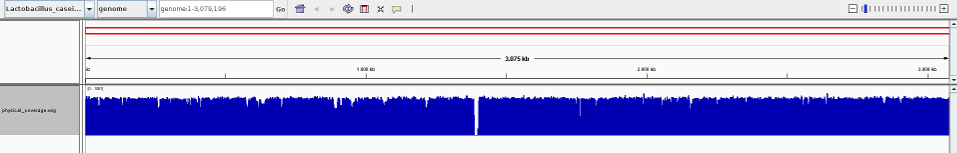
\includegraphics[scale=0.6]{immagini/physical_coverage_1.png}
				\caption{Whole sequence coverage}\label{fig:6}
				\end{figure}


 \begin{figure}[H]
				\centering
				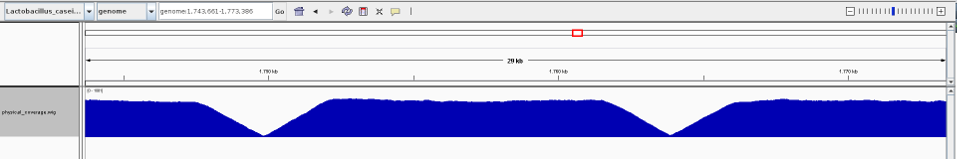
\includegraphics[scale=0.6]{immagini/physical_coverage_2.png}
				\caption{sequence coverage, in the same position the physiscal coverage identify an inversion structural modification}\label{fig:7}
				\end{figure}
				
				
				
 \begin{figure}[H]
				\centering
				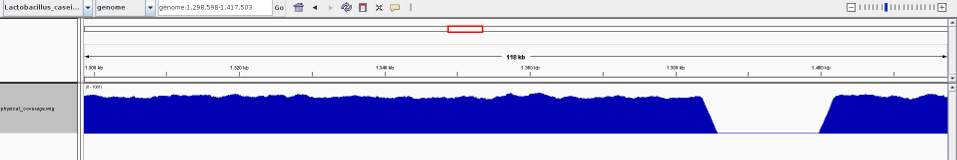
\includegraphics[scale=0.6]{immagini/physical_coverage_3.png}
				\caption{Sequence coverage that identify an structural variation, exactly a long deletation}\label{fig:8}
				\end{figure}				


\section{Sequence Coverage}
The Sequence Coverage is calulated by the algorithm contained inside the SequenceCoverageAlgorithm.py.\\
This algorithm is similar to the physical coverage script's but with the differences who is necessary the read that has positive and negative \emph{TLEN}.\\
As well the Physical coverage, also, this algorithm make a check on the \emph{FLAG} field
\\
\\

At first time, I had created an array where each cell was be intialized to 0.
Then for each cell that has with the index between START to START + sequence lenght, I put +1.
This step is necessary for each compatible reads.\\\\

The resultant values were putted inside a wig file, called \emph{sequeence\_coverage.wig}.

After that the file was loaded onto IGV to show the sequence coverage to help to make hypotesys and analisys about some structural variations.

Some small part of resultant traks produced by the IGV are reported below:


 \begin{figure}[H]
				\centering
				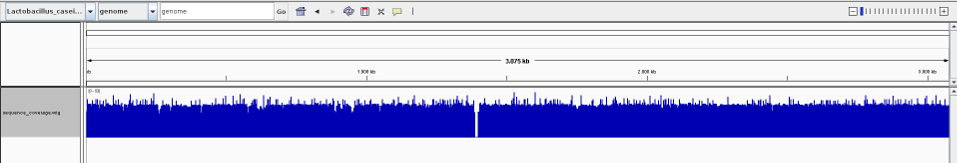
\includegraphics[scale=0.6]{immagini/sequence_coverage_1.png}
				\caption{Whole physical coverage}\label{fig:9}
				\end{figure}


 \begin{figure}[H]
				\centering
				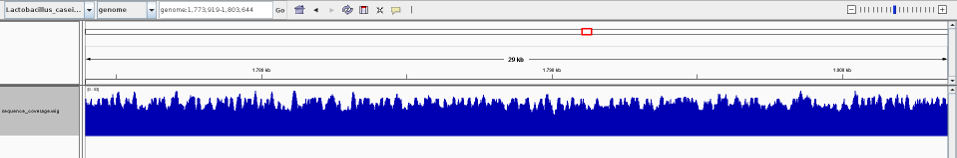
\includegraphics[scale=0.6]{immagini/sequence_coverage_2.png}
				\caption{Physical coverage that identify an structural variation}\label{fig:10}
				\end{figure}
				
				
				
 \begin{figure}[H]
				\centering
				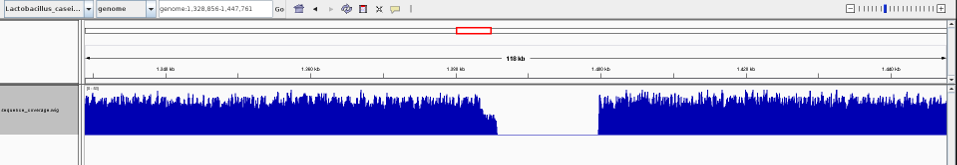
\includegraphics[scale=0.6]{immagini/sequence_coverage_3.png}
				\caption{Physical coverage that identify an structural variation}\label{fig:11}
				\end{figure}	
\section{Kmers counting}
To start talking about the kmers, is necessay to define what is it.
\begin{quote}
The term k-mer typically refers to all the possible substrings of length k that are contained in a string. In computational genomics, k-mers refer to all the possible subsequences (of length k) from a read obtained through DNA Sequencing
\end{quote}

The algorithm for the kmers analisys is inside the KmersAlgorithm.py.\\
to work, the algorithm expects the kmers length value, many different test was made using 7-mers, 4-mers and 9-mers.\\
The result was be really different and to make some hypotesys or analisys was be necessary plot different barchart by usign some R scripts.\\\\

These traks has allowed to learn and see what are the most, and the less present kmers inside the resequenced genome.\\

The algorithm consider each kmers with the relative opposite, the goal is eliminate the errors that could comes from the "string slicing" from the kmers build.\\\\

The algorithm start from position 0 of each \emph{SEQ} and terminate with the end of \emph{SEQ}.
In each loop made on the SEQ string, the algorithm move the start position from \verb|i| to \verb|i+1| and the end position from \verb|end| to \verb|end+1|.\\
The resultant substring is exactly long how we aspect.\\\\

I reported the traks generated by the different k dimensions below:

 \begin{figure}[H]
				\centering
				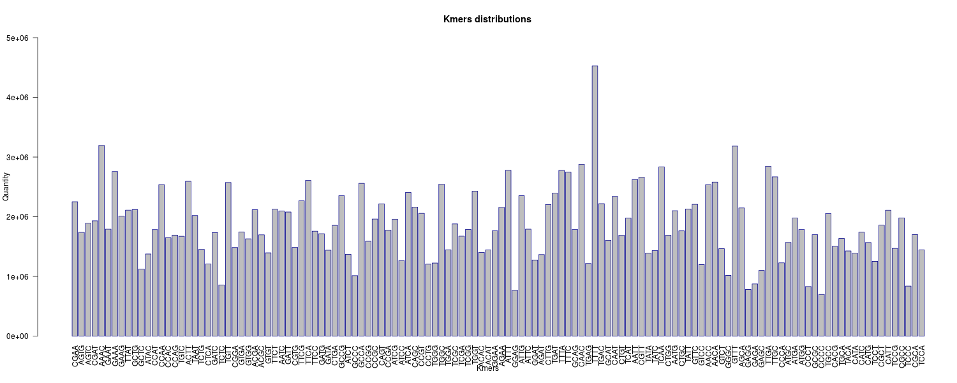
\includegraphics[scale=0.45]{immagini/kmers_4.png}
				\caption{Kmers with k = 4}\label{fig:12}
				\end{figure}


 \begin{figure}[H]
				\centering
				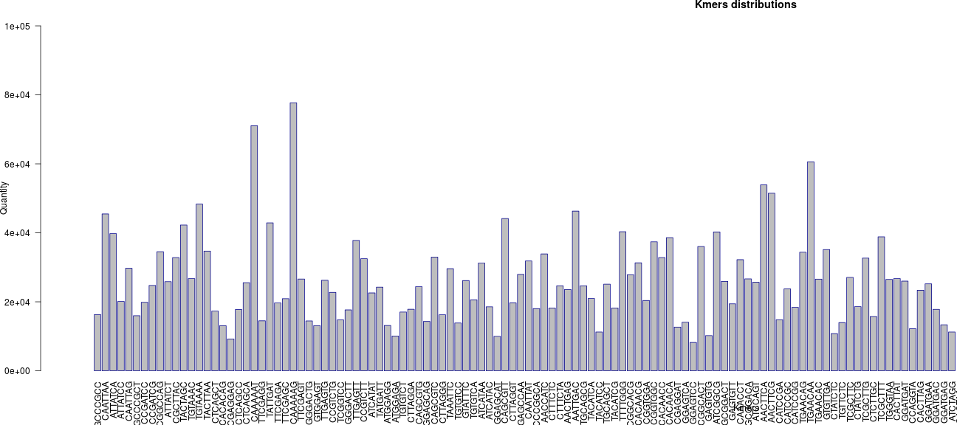
\includegraphics[scale=0.45]{immagini/kmers_7.png}
				\caption{Kmers with k = 7}\label{fig:13}
				\end{figure}
				
				
				
 \begin{figure}[H]
				\centering
				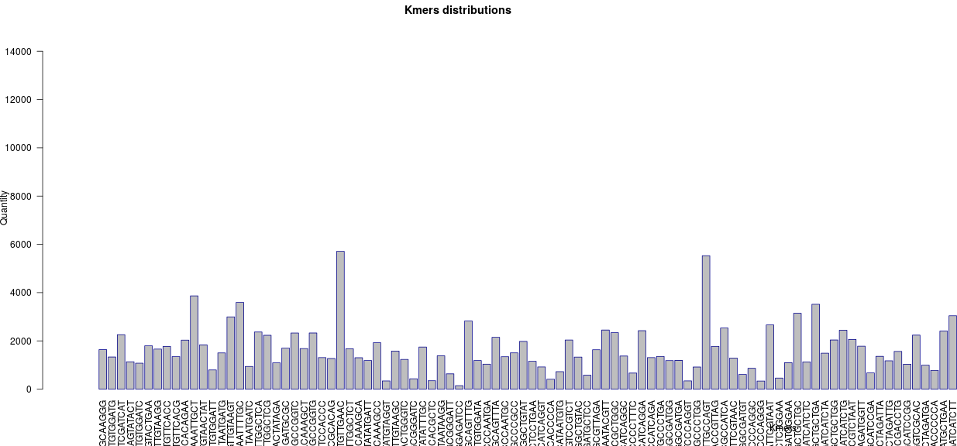
\includegraphics[scale=0.45]{immagini/kmers_9.png}
				\caption{Kmers with k = 9}\label{fig:14}
				\end{figure}	
				
In these traks is simple to see what kmers are more frequent then others, the observation of the kmers and the relative bases should be helpfull for the gene recongition, because should allows the reasearch of a certain protein.				

\section{Cigar H and S reads}             % Processi
% !TEX encoding = UTF-8
% !TEX TS-program = pdflatex
% !TEX root = ../tesi.tex
% !TEX spellcheck = it-IT

%**************************************************************
\chapter{Descrizione dello stage}
\label{cap:descrizione-stage}
%**************************************************************

\intro{Breve introduzione al capitolo}\\

%**************************************************************
\section{Introduzione al progetto}

%**************************************************************
\section{Analisi preventiva dei rischi}

Durante la fase di analisi iniziale sono stati individuati alcuni possibili rischi a cui si potrà andare incontro.
Si è quindi proceduto a elaborare delle possibili soluzioni per far fronte a tali rischi.\\

\begin{risk}{Performance del simulatore hardware}
    \riskdescription{le performance del simulatore hardware e la comunicazione con questo potrebbero risultare lenti o non abbastanza buoni da causare il fallimento dei test}
    \risksolution{coinvolgimento del responsabile a capo del progetto relativo il simulatore hardware}
    \label{risk:hardware-simulator} 
\end{risk}

%**************************************************************
\section{Requisiti e obiettivi}


%**************************************************************
\section{Pianificazione}             % Kick-Off
% !TEX encoding = UTF-8
% !TEX TS-program = pdflatex
% !TEX root = ../tesi.tex
% !TEX spellcheck = it-IT

%**************************************************************
\chapter{Considerations}
\label{cap:considerations}
%**************************************************************

\intro{Breve introduzione al capitolo}\\

\section{Considerations}
             % Concept Preview
% !TEX encoding = UTF-8
% !TEX TS-program = pdflatex
% !TEX root = ../tesi.tex
% !TEX spellcheck = it-IT

%**************************************************************
\chapter{Progettazione e codifica}
\label{cap:progettazione-codifica}
%**************************************************************

\intro{Breve introduzione al capitolo}\\

%**************************************************************
\section{Tecnologie e strumenti}
\label{sec:tecnologie-strumenti}

Di seguito viene data una panoramica delle tecnologie e strumenti utilizzati.

\subsection*{Tecnologia 1}
Descrizione Tecnologia 1.

\subsection*{Tecnologia 2}
Descrizione Tecnologia 2

%**************************************************************
\section{Ciclo di vita del software}
\label{sec:ciclo-vita-software}

%**************************************************************
\section{Progettazione}
\label{sec:progettazione}

\subsubsection{Namespace 1} %**************************
Descrizione namespace 1.

\begin{namespacedesc}
    \classdesc{Classe 1}{Descrizione classe 1}
    \classdesc{Classe 2}{Descrizione classe 2}
\end{namespacedesc}


%**************************************************************
\section{Design Pattern utilizzati}

%**************************************************************
\section{Codifica}
             % Product Prototype
% !TEX encoding = UTF-8
% !TEX TS-program = pdflatex
% !TEX root = ../tesi.tex
% !TEX spellcheck = it-IT

%**************************************************************
\chapter{Verifica e validazione}
\label{cap:verifica-validazione}
%**************************************************************             % Product Design Freeze e SOP
% !TEX encoding = UTF-8
% !TEX TS-program = pdflatex
% !TEX root = ../tesi.tex
% !TEX spellcheck = it-IT

%**************************************************************
\chapter{Conclusioni}
\label{cap:conclusioni}
%**************************************************************

%**************************************************************
\section{Consuntivo finale}

%**************************************************************
\section{Raggiungimento degli obiettivi}

%**************************************************************
\section{Conoscenze acquisite}

%**************************************************************
\section{Valutazione personale}
             % Conclusioni
\appendix                               
% !TEX encoding = UTF-8
% !TEX TS-program = pdflatex
% !TEX root = ../tesi.tex
% !TEX spellcheck = it-IT

%**************************************************************
\chapter{Appendice A}
%**************************************************************

\epigraph{Citazione}{Autore della citazione}



             % Appendice A

%**************************************************************
% Materiale finale
%**************************************************************
\backmatter
\printglossaries
%% !TEX encoding = UTF-8
% !TEX TS-program = pdflatex
% !TEX root = ../tesi.tex
% !TEX spellcheck = it-IT

%**************************************************************
% Bibliografia
%**************************************************************

\cleardoublepage
\chapter{Bibliografia}

\nocite{*}
%\printbibliography

\bibbycategory % equivale a dare un \printbibliography per ogni categoria


\end{document}